\documentclass[]{book}

%These tell TeX which packages to use.
\usepackage{array,epsfig}
\usepackage{amsmath}
\usepackage{amsfonts}
\usepackage{amssymb}
\usepackage{amsxtra}
\usepackage{amsthm}
\usepackage{mathrsfs}
\usepackage{color}
\usepackage{graphicx}

%Here I define some theorem styles and shortcut commands for symbols I use often
\theoremstyle{definition}
\newtheorem{defn}{Definition}
\newtheorem{thm}{Theorem}
\newtheorem{cor}{Corollary}
\newtheorem*{rmk}{Remark}
\newtheorem{lem}{Lemma}
\newtheorem*{joke}{Joke}
\newtheorem{ex}{Example}
\newtheorem*{soln}{Solution}
\newtheorem{prop}{Proposition}

\newcommand{\lra}{\longrightarrow}
\newcommand{\ra}{\rightarrow}
\newcommand{\surj}{\twoheadrightarrow}
\newcommand{\graph}{\mathrm{graph}}
\newcommand{\bb}[1]{\mathbb{#1}}
\newcommand{\Z}{\bb{Z}}
\newcommand{\Q}{\bb{Q}}
\newcommand{\R}{\bb{R}}
\newcommand{\C}{\bb{C}}
\newcommand{\N}{\bb{N}}
\newcommand{\M}{\mathbf{M}}
\newcommand{\m}{\mathbf{m}}
\newcommand{\MM}{\mathscr{M}}
\newcommand{\HH}{\mathscr{H}}
\newcommand{\Om}{\Omega}
\newcommand{\Ho}{\in\HH(\Om)}
\newcommand{\bd}{\partial}
\newcommand{\del}{\partial}
\newcommand{\bardel}{\overline\partial}
\newcommand{\textdf}[1]{\textbf{\textsf{#1}}\index{#1}}
\newcommand{\img}{\mathrm{img}}
\newcommand{\ip}[2]{\left\langle{#1},{#2}\right\rangle}
\newcommand{\inter}[1]{\mathrm{int}{#1}}
\newcommand{\exter}[1]{\mathrm{ext}{#1}}
\newcommand{\cl}[1]{\mathrm{cl}{#1}}
\newcommand{\ds}{\displaystyle}
\newcommand{\vol}{\mathrm{vol}}
\newcommand{\cnt}{\mathrm{ct}}
\newcommand{\osc}{\mathrm{osc}}
\newcommand{\LL}{\mathbf{L}}
\newcommand{\UU}{\mathbf{U}}
\newcommand{\support}{\mathrm{support}}
\newcommand{\AND}{\;\wedge\;}
\newcommand{\OR}{\;\vee\;}
\newcommand{\Oset}{\varnothing}
\newcommand{\st}{\ni}
\newcommand{\wh}{\widehat}

%Pagination stuff.
\setlength{\topmargin}{-.3 in}
\setlength{\oddsidemargin}{0in}
\setlength{\evensidemargin}{0in}
\setlength{\textheight}{9.in}
\setlength{\textwidth}{6.5in}
\pagestyle{empty}



\begin{document}


\begin{center}
{\Large The gambler's ruin \hspace{0.5cm} Part 1 (two-player)}\\
\textbf{Alireza Abrehforoush}\\ %You should put your name here
Date: 6/29/2022 %You should write the date here.
\end{center}

\vspace{0.2 cm}


\section*{Recursion}
\subsection*{Model}
\begin{figure}[h]
    \centering
    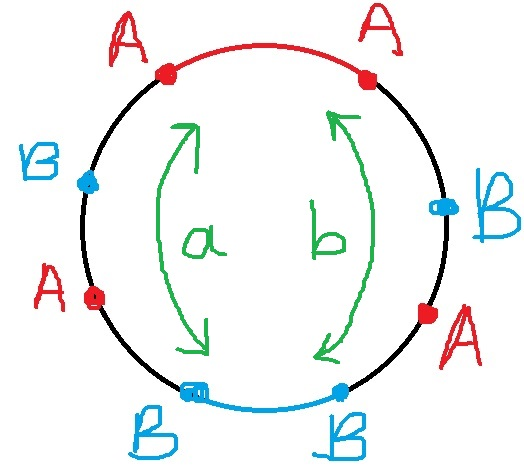
\includegraphics[width=0.25\textwidth]{model1.jpg}
    \caption{two-player with $k=8$ and initial value of $a$ and $b$ for players}
    \label{fig:mesh1}
\end{figure}


\subsection*{Definition}
%%%%%%%%%%%%%%%%%%%%%%%%%%%%%%%%%%%
%Define the \textdf{$\ell^1$-norm} on $\R^n$ by
%	$$\|x\|_1 = \sum_{i=1}^n |x^i|,$$
%	and define the \textdf{sup-norm} on $\R^n$ by
%	$$\|x\|_\infty = \sup\left\{|x^i|\right\}.$$
%	Show that these satisfy Theorem~1.
%%%%%%%%%%%%%%%%%%%%%%%%%%%%%%%%%%%
$$
t_{a} := expected \hspace{0.2cm} duration \hspace{0.2cm} of \hspace{0.2cm} game \hspace{0.2cm} starting \hspace{0.2cm} from \hspace{0.2cm} a
\newline
$$

$$t_{a} = \frac{1}{2}t_{a-1} + \frac{1}{2}t_{a+1} + 1 \newline$$

$$
\Rightarrow t_{a+1} = 2t_{a} - t_{a-1} - 2 \newline
$$

$$
\Rightarrow t_{a} = 2t_{a-1} - t_{a-2} - 2
$$
	
\subsection*{Initial values}
\subsubsection*{mine}
$$
\begin{cases}
  t_{0} = 0 \\
  t_{k} = 0
\end{cases}
$$

\subsubsection*{yours}
$$
\begin{cases}
  t_{0} = 0 + \frac{2}{k}t_{1} + 1 \\
  X_{k} = 0
\end{cases}
$$

\subsection*{Solving recurrence}
\subsubsection*{mine}
$$
r^2 -2r + 1 = 0 \newline
$$
$$
\Rightarrow t^{(h)}_{a} = \alpha_{1} + \alpha_{2}n
$$

\subsubsection*{yours}
$$
-2\alpha^2 + \alpha + 2 = 0 \newline
$$
$$
\Rightarrow \alpha = \frac{-1\pm \sqrt{1+16}}{-4} \newline
$$



\begin{proof}
	% WRITE YOUR PROOF HERE.
\end{proof}





\end{document}


